\documentclass[dvipsnames,usenames,10pt]{beamer}

\usetheme{JuanLesPins}

\title{A Multi-Agent System for playing Briscola Chiamata} 

\author[B. Borja Fiz, F. De Santis, M. Gabarda]{Beltran Borja Fiz, Fabrizio De Santis, Marcos Gabarda}
\institute[Universitat Polit\`ecnica de Catalunya]{
			Multi-agent Systems Course\\
			Master in Artificial Intelligence\\
			Universitat Polit\`ecnica de Catalunya\\
			\texttt{\\ \{beltran.borja.fiz, fabrizio.de.santis, marcos.gabarda\}@est.fib.upc.edu}}
\date{\today}

\begin{document}

\frame{\titlepage}

\section*{Outline}

\frame{
	\frametitle{Outline}
	\tableofcontents
}

\frame[allowframebreaks]{
  \frametitle{Introduction}
\begin{itemize}
  \item Briscola Chiamata
  \item Prometheus methodology (PDT Tool)
  \item 2APL
  \item ...
\end{itemize}
}

\section{Problem Specification}

\frame[allowframebreaks]{
    \frametitle{A bit of terminology}
  
    \begin{itemize}
      \item Game:
      \item Hand/Turn:
      \item Trick:
      \item Suit:
      \item Rank:
      \item Briscola:
    \end{itemize}
}

\frame[allowframebreaks]{
    \frametitle{Briscola Chiamata}

    5 players, 8 cards each, no cards undealt

    \vskip 2.0ex

    Phases of the game:
    \begin{itemize}  
      \item Card giving
      \item Bidding
      \item Partner selection
      \item Playing cards
      \item Winner/Loser declaration with point distribution
    \end{itemize}
}


\frame[allowframebreaks]{
  \frametitle{Why is suitable for MAS?}

  \begin{itemize}
    \item Uncertainity (nobody knows who is actually its partner)
    \item Sociality (its needed in order to discover partners/cheat opponents)
    \item Coordination is needed
    \begin{itemize}
      \item Cooperation inside teams needed once partners are discovered
      \item Competition between teams needed once partners are discovered
    \end{itemize}
    \item Trust/Reputation models needed 
    \item Main agent properties are satisfied
    \begin{itemize}
      \item Autonomy (players are autonomous, they plan alone once there are at least 5 players)
      \item Flexibility
      \item Reactivity (players has to play when its their turn)
      \item Proactivity (players can decide if they want to play even if it's not their turn, players can decide to start cheating other players by sending them messages)
      \item Social (players have to interact with each others in order to discover their partners)
    \end{itemize}
  \end{itemize}

%     Uncertainity (nobody knows who is actually its partner)
%     Sociality (its needed in order to discover partners/cheat opponents)
%     Coordination is needed that is:
%       Cooperation inside teams needed once partners are discovered
%       Competition between teams needed once partners are discovered
%     Trust/Reputation models needed 
%     
%     Main agent properties are satisfied:
%       Autonomy (players are autonomous, they plan alone once there are at least 5 players)
%       Flexibility that is:
%          Reactivity (players has to play when its their turn)
%          Proactivity (players can decide if they want to play even if it's not their turn, players can decide to start cheating other players by sending them messages)
%          Social (players have to interact with each others in order to discover their partners)
}

\section{System Specification}

\frame[allowframebreaks]{
  \frametitle{Analysis Overview Diagram}

  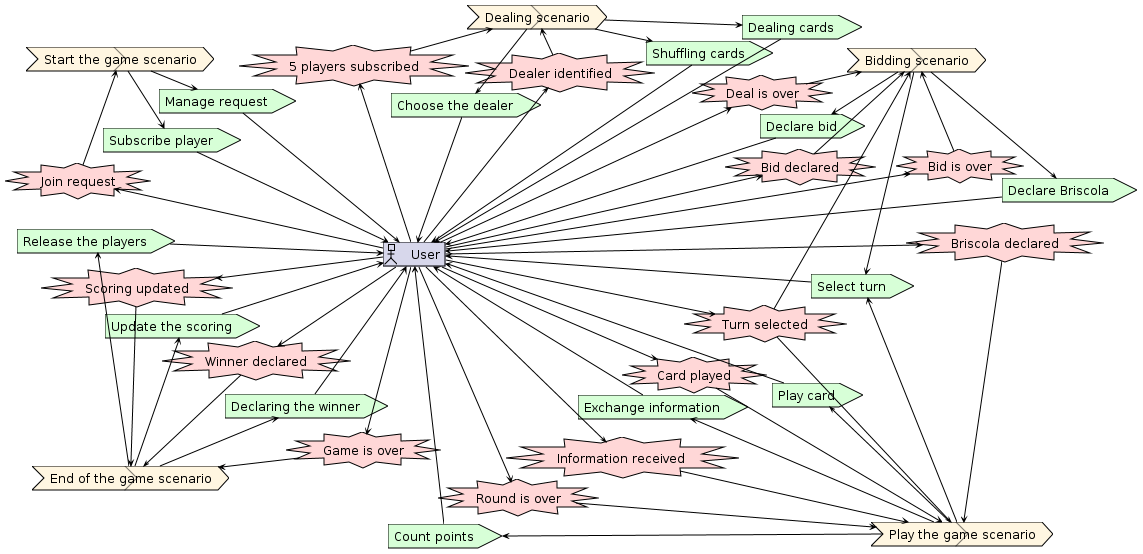
\includegraphics[keepaspectratio,scale=0.3]{pdt/images/system_specification/analysis_overview.png}

}

\frame[allowframebreaks]{
  \frametitle{Scenarios Diagram}

  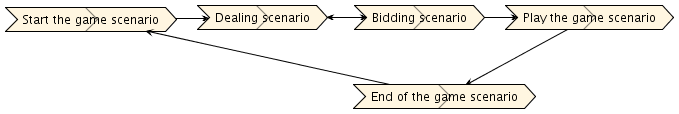
\includegraphics[keepaspectratio,scale=0.3]{pdt/images/system_specification/scenarios.png}

}

\frame[allowframebreaks]{
  \frametitle{Goals Overview Diagram}

  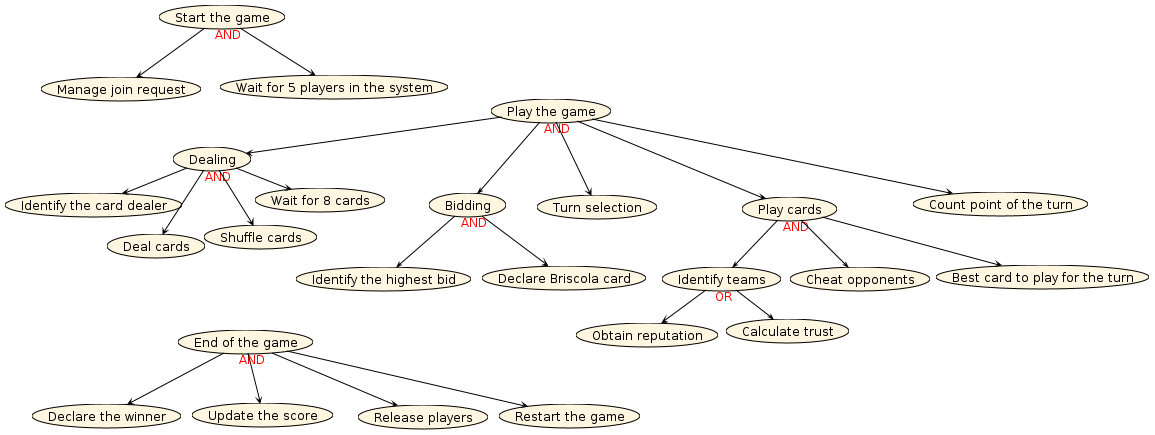
\includegraphics[keepaspectratio,scale=0.3]{pdt/images/system_specification/goal_overview.png}

}

\frame[allowframebreaks]{
  \frametitle{System Roles Diagram}

  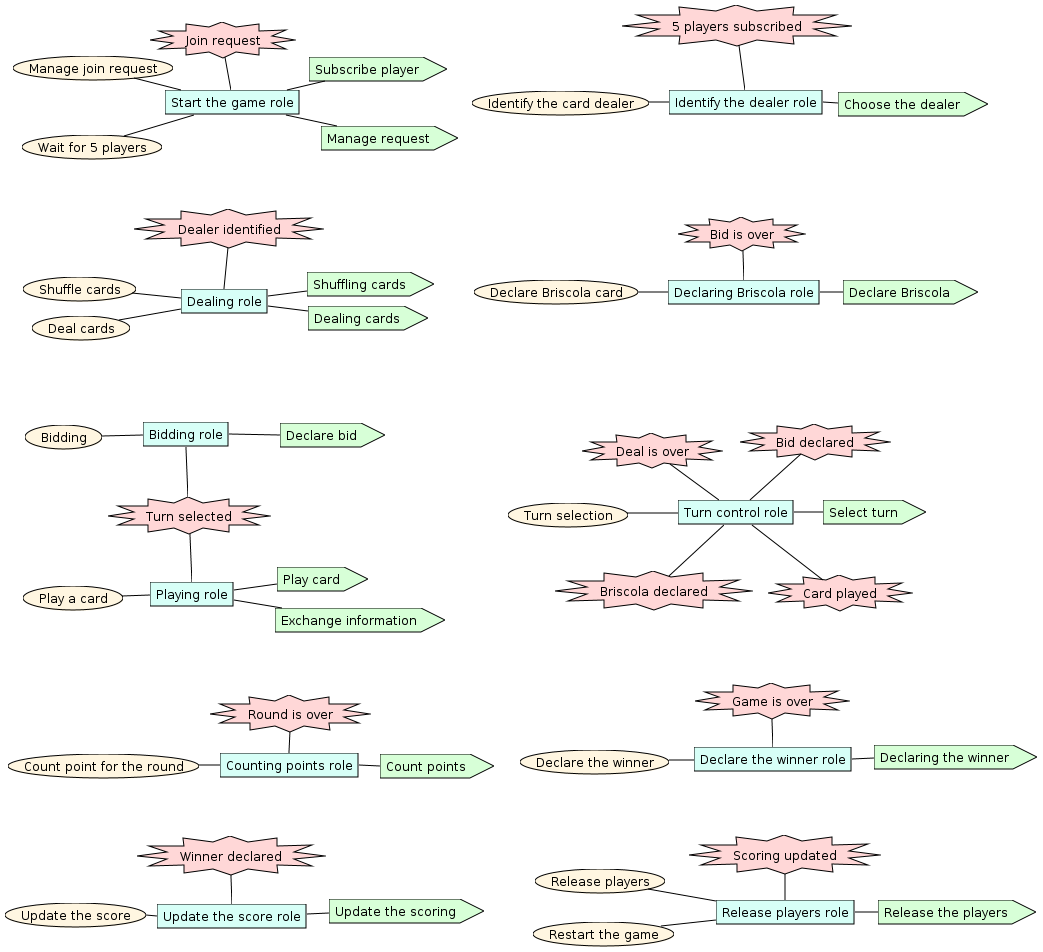
\includegraphics[keepaspectratio,scale=0.3]{pdt/images/system_specification/system_roles.png}

}

\section{High-level (Architectural) Design}

\frame[allowframebreaks]{
  \frametitle{Data Coupling Diagram}

  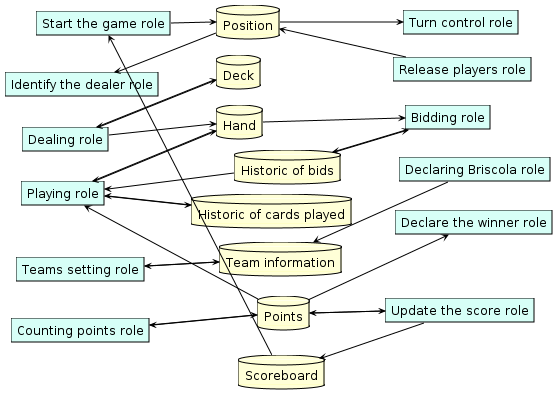
\includegraphics[keepaspectratio,scale=0.3]{pdt/images/architectural_design/data_coupling.png}

}

\frame[allowframebreaks]{
  \frametitle{Agent-Role Grouping Diagram}

  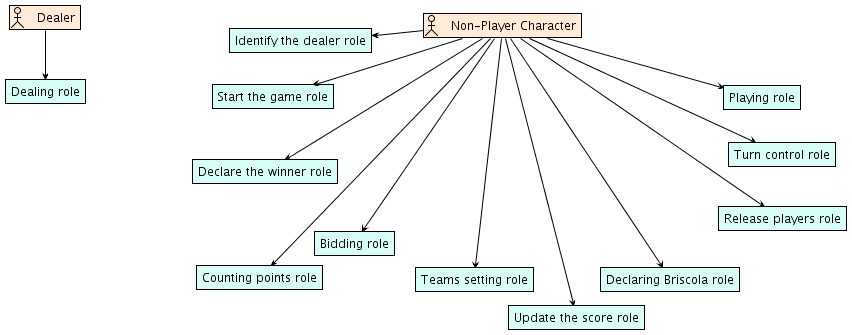
\includegraphics[keepaspectratio,scale=0.3]{pdt/images/architectural_design/aget-role_grouping.png}

}

\frame[allowframebreaks]{
  \frametitle{Agent Acquaintance Diagram}

  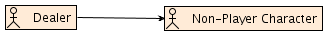
\includegraphics[keepaspectratio,scale=0.3]{pdt/images/architectural_design/agent_acquaintance.png}

}

\frame[allowframebreaks]{
  \frametitle{System Overview Diagram}

  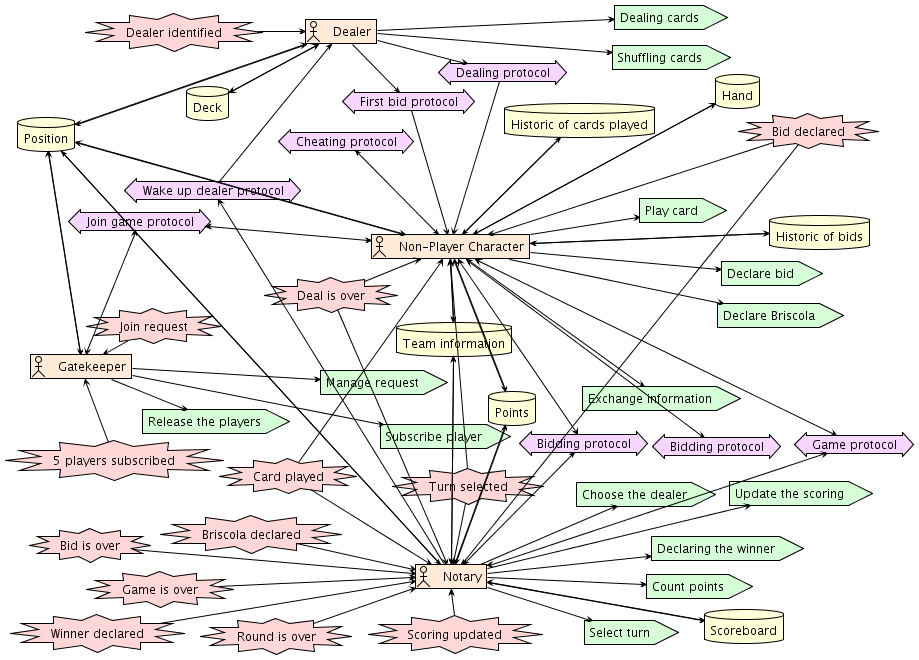
\includegraphics[keepaspectratio,scale=0.3]{pdt/images/architectural_design/system_overview.png}

}

\section{Detailed Design}

\frame[allowframebreaks]{
  \frametitle{Agent Overview Diagram}

  
}

\frame[allowframebreaks]{
  \frametitle{Capability Overview Diagram}

  
}


\frame[allowframebreaks]{
  \frametitle{Conclusion}

  What's wrong with 2APL?

  No security mechanisms
}


\begin{frame}{Bibliography}
\nocite{*}
\bibliographystyle{plain}
\bibliography{bc-pres}
\end{frame}

\end{document}
